%!TeX root=../tese.tex
%("dica" para o editor de texto: este arquivo é parte de um documento maior)

% Conteúdo da subseção sobre Remuneração
% Este arquivo é importado em 02-implementacao.tex

A Lei Municipal 16.547/2016 estabeleceu
que o pagamento aos ciclistas do programa BikeSP seria realizado através de créditos
de transporte público, inseridos diretamente nos cartões Bilhete Único dos
participantes. Esta escolha reflete a intenção do governo municipal de integrar a
bicicleta ao sistema de transporte público, permitindo que os incentivos sejam
utilizados para deslocamentos multimodais (bicicleta + ônibus/metrô). O modelo de
remuneração por quilômetro pedalado, adotado também em iniciativas internacionais
como em Itajaí e na Holanda \citep{itajai2021, tennant2022}, visa recompensar a distância economizada ao
substituir outros modos de transporte, facilitando análises de impacto em poluição,
tráfego e saúde pública.

No desenho experimental do piloto, optou-se por valores de R\$~0,30 e R\$~0,60 por
quilômetro (equivalentes a 1/16 e 1/8 de uma passagem de transporte público,
respectivamente), com limite de duas viagens remuneradas por dia. Estes valores foram
baseados em estudo do Banco Mundial sobre disposição a pagar por ciclismo em São
Paulo \citep{worldbank2022}, que identificou que remunerações entre R\$~2,00 e R\$~3,00 por viagem
aumentavam em 38,4\% a probabilidade de escolher bicicleta sobre o modo atual,
efeito comparável à presença de ciclovias (43,4\%). A remuneração não foi
diferenciada por perfil de participante durante o piloto, pois um dos objetivos do
experimento era justamente compreender como o impacto da remuneração varia
segundo diferentes perfis demográficos e socioeconômicos.

O sistema de remuneração implementado no
painel administrativo gerencia três estados distintos do dinheiro: (i)
\texttt{aguardandoEnvio} --- valores de viagens aprovadas, bônus concedidos e
contestações deferidas que ainda não foram enviados à SPTrans; (ii)
\texttt{aguardandoResposta} --- valores já enviados à SPTrans através de arquivo
CSV, aguardando confirmação de creditação; e (iii) \texttt{concedido} --- valores
confirmados pela SPTrans como efetivamente creditados nos cartões Bilhete Único dos
participantes. Esta separação em estados permite rastreabilidade completa do fluxo
financeiro e reconciliação precisa entre solicitações, confirmações e valores
efetivamente pagos.

A funcionalidade de geração de CSV
para pagamento compila todos os valores em estado \texttt{aguardandoEnvio} de
participantes com Bilhete Único ativo. O arquivo gerado segue formato específico
exigido pela SPTrans: duas colunas delimitadas por ponto e vírgula (número do
Bilhete Único e valor), sem cabeçalho. O nome do arquivo inclui data e hora completa (exemplo:
\texttt{pagamentos05-10-2024-14-30-25.csv}) para garantir unicidade e
rastreabilidade. Ao gerar o CSV, o sistema automaticamente move os valores de
\texttt{aguardandoEnvio} para \texttt{aguardandoResposta}, evitando duplicação em
envios subsequentes. Esta operação é atômica e registrada em log para auditoria. A Figura~\ref{fig:remuneracao_gerar_csv_form_creditos} mostra a interface de geração.

\begin{figure}[H]
    \centering
    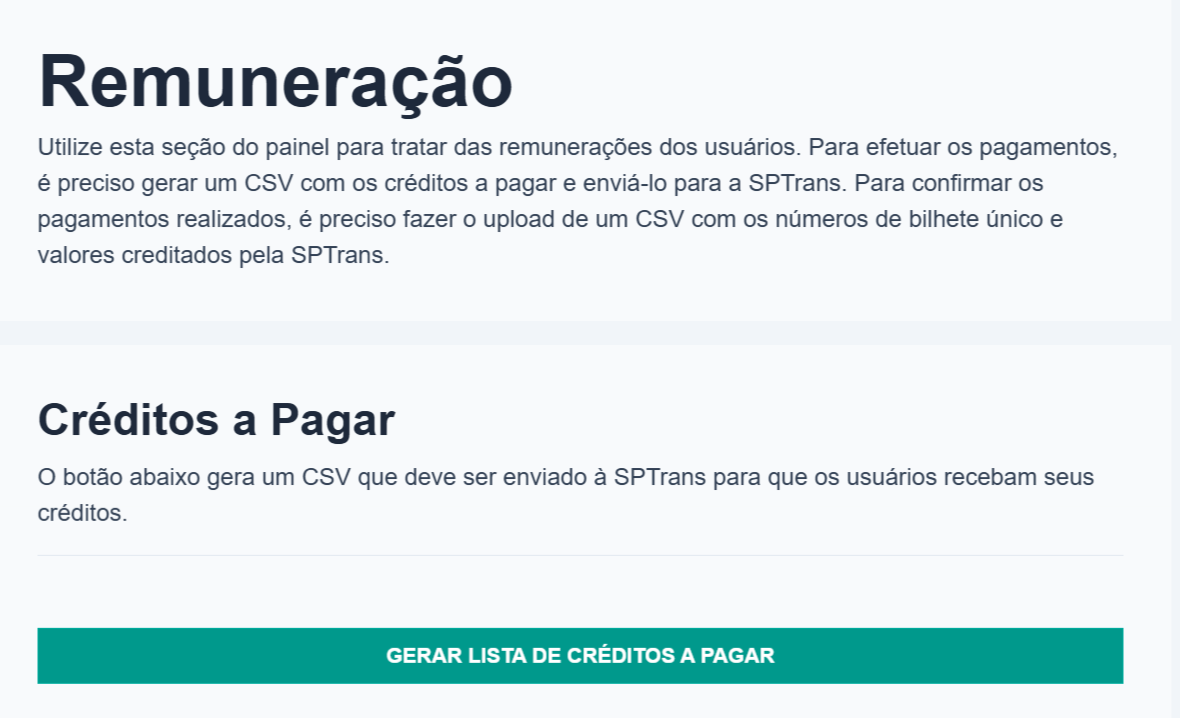
\includegraphics[width=0.95\textwidth]{figuras/remuneracao_creditos.png}
    \caption{Interface de geração de lista de créditos a pagar via SPTrans.}
    \label{fig:remuneracao_gerar_csv_form_creditos}
  \end{figure}

O arquivo CSV gerado é enviado
manualmente à SPTrans. A SPTrans credita os valores nos cartões Bilhete
Único dos participantes e retorna um arquivo CSV de comprovação contendo os bilhetes
efetivamente creditados e os valores pagos. Este processo manual, embora não
automatizado, mostrou-se adequado para a escala do piloto (cerca de 1.200
participantes) e garante supervisão humana sobre transações financeiras, reduzindo
riscos de erros sistêmicos em larga escala.



Ao receber o comprovante da SPTrans,
o administrador realiza upload do arquivo CSV no painel. O sistema executa validação
rigorosa linha por linha: verifica formato (exatas duas colunas), existência do
Bilhete Único no banco de dados, e validade numérica do valor. Qualquer erro
detectado aborta imediatamente o processamento completo, impedindo confirmações
parciais que poderiam gerar inconsistências. Apenas quando todas as linhas são
validadas com sucesso, o sistema processa a confirmação: move valores de
``aguardando resposta'' para ``concedido'', registra o histórico de pagamento como confirmado, e armazena a data e valor de cada operação. Mensagens específicas de erro (``Arquivo com
mais de duas colunas'', ``Formato incorreto de valor'', ``Bilhete não encontrado'')
facilitam correção rápida de problemas antes de reprocessar. A Figura~\ref{fig:remuneracao_gerar_csv_form_processados} ilustra a interface de upload.

\begin{figure}[H]
    \centering
    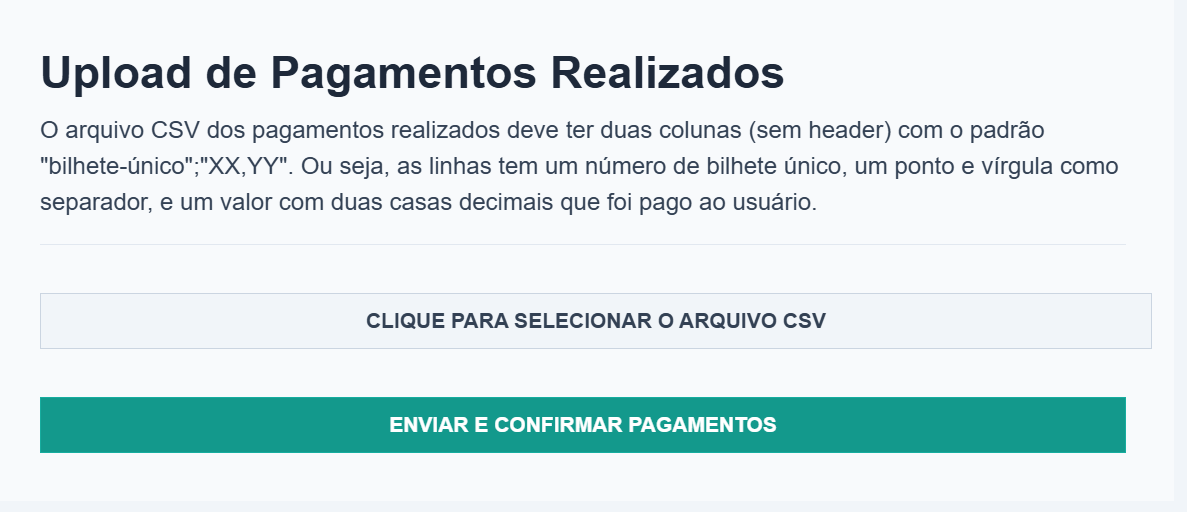
\includegraphics[width=0.95\textwidth]{figuras/remuneracao_processados.png}
    \caption{Interface de upload de comprovante de pagamentos realizados pela SPTrans.}
    \label{fig:remuneracao_gerar_csv_form_processados}
  \end{figure}
O sistema armazena, para cada Bilhete Único, os três estados de remuneração (concedido, aguardando envio, aguardando resposta) além da identificação do participante e status de ativação do cartão. Mantém também registro imutável de todos os envios de pagamento (identificados por número do bilhete e data), permitindo múltiplos pagamentos ao mesmo participante ao longo do tempo. Restrições do banco de dados garantem que valores sejam sempre não
negativos e que transições de estado sigam apenas fluxos
válidos. Toda operação financeira é registrada em log incluindo ID do administrador
responsável, garantindo trilha de auditoria completa e rastreabilidade para
conformidade com procedimentos do experimento.

O painel oferece visibilidade
sobre valores pendentes de envio, valores aguardando confirmação da SPTrans, e total pago aos participantes. 
Durante o piloto, estes indicadores foram fundamentais para
planejamento de fluxo de caixa e comunicação com participantes sobre prazos
esperados de creditação. 

O sistema contempla cenários
atípicos que ocorreram durante operação: (i) pagamentos parciais, quando SPTrans
credita valor inferior ao solicitado, mantendo diferença pendente de confirmação para reenvio posterior; (ii) bilhetes inválidos ou
bloqueados, que não aparecem no CSV de retorno da SPTrans e requerem investigação
manual com o participante; (iii) múltiplos pagamentos no mesmo dia, permitidos via
timestamp distinto na chave primária; e (iv) valores zerados no CSV, que são
ignorados sem gerar erro. A natureza atômica e idempotente do processamento de
confirmações permite reprocessar o mesmo CSV sem duplicações, útil em casos de
falhas de comunicação ou necessidade de revalidação.


